\documentclass{article}
\usepackage{graphicx}
\usepackage[dvipsnames,table]{xcolor}
\usepackage[utf8]{inputenc}
\usepackage{siunitx}
\usepackage[american,siunitx]{circuitikz}
\usepackage{amsmath}
\usepackage{svg}
\usepackage{booktabs}
\usepackage{float}
\usepackage{xparse, xfp}
\usepackage{multirow}
\usepackage{tikz}
\usepackage{karnaugh-map}
\usepackage{pdfpages}
\usepackage{hyperref}
\hypersetup{
    colorlinks=true,
    linkcolor=blue,
    filecolor=magenta,      
    urlcolor=cyan,
}
\usepackage{caption} 

\makeatletter
\ctikzset{lx/.code args={#1 and #2}{ 
  \pgfkeys{/tikz/circuitikz/bipole/label/name=\parbox{1cm}{\centering #1  \\ #2}}
    \ctikzsetvalof{bipole/label/unit}{}
    \ifpgf@circ@siunitx 
        \pgf@circ@handleSI{#2}
        \ifpgf@circ@siunitx@res 
            \edef\pgf@temp{\pgf@circ@handleSI@val}
            \pgfkeyslet{/tikz/circuitikz/bipole/label/name}{\pgf@temp}
            \edef\pgf@temp{\pgf@circ@handleSI@unit}
            \pgfkeyslet{/tikz/circuitikz/bipole/label/unit}{\pgf@temp}
        \else
        \fi
    \else
    \fi
}}

\ctikzset{lx^/.style args={#1 and #2}{ 
    lx=#2 and #1,
    \circuitikzbasekey/bipole/label/position=90 } 
}

\ctikzset{lx_/.style args={#1 and #2}{ 
    lx=#1 and #2,
    \circuitikzbasekey/bipole/label/position=-90 } 
}
\makeatother

\captionsetup[table]{skip=10pt}

\usetikzlibrary{calc}
%\usepackage[landscape]{geometry}
\renewcommand{\thesubsection}{\thesection.\alph{subsection}}
\newcommand{\equal}{=}
\newcommand{\greyrule}{\arrayrulecolor{black!30}\midrule\arrayrulecolor{black}}
\makeatletter
\newcommand\currcoor{\the\tikz@lastxsaved,\the\tikz@lastysaved}
\makeatother
\newcolumntype{:}{@{\hskip\tabcolsep\color{black!30}\vrule\hskip\tabcolsep}}

\ExplSyntaxOn
\NewExpandableDocumentCommand \groupify { O{\,\allowbreak} m m }
  { \jakob_groupify:nnn {#1} {#2} {#3} }
\cs_new:Npn \jakob_groupify:nnn #1 #2 #3
  { \__jakob_groupify_loop:nnw { 1 } {#2} #3 \q_recursion_tail {#1} \q_recursion_stop }
\cs_new:Npn \__jakob_groupify_loop:nnw #1 #2 #3
  {
    \quark_if_recursion_tail_stop:n {#3}
    \exp_not:n {#3}
    \int_compare:nNnTF {#1} = {#2}
      { \__jakob_groupify_sep:n }
      { \exp_args:Nf \__jakob_groupify_loop:nnw { \int_eval:n { #1+1 } } }
          {#2}
  }
\cs_new:Npn \__jakob_groupify_sep:n #1 #2 \q_recursion_tail #3
  {
    \tl_if_empty:nF {#2} { \exp_not:n {#3} }
    \__jakob_groupify_loop:nnw { 1 } {#1}
    #2 \q_recursion_tail {#3}
  }
\ExplSyntaxOff

\title{ECE 2200L\\Introduction to Microelectronics Circuits Laboratory\\\,\\Experiment 9\\MOSFET and BJT Logic Inverters\\\,\\Report}
\author{Choi Tim Antony Yung}
\date{November 4, 2020}
\begin{document}
\maketitle

\thispagestyle{empty}
\setcounter{page}{0}

\newpage

\section*{Objective}
To study the applications of MOSFET and BJT devices to digital logic circuits.  A MOSFET gate inverter and a BJT base inverter will be investigated.

\section*{Result}

\begin{figure}[H]
  \centering
  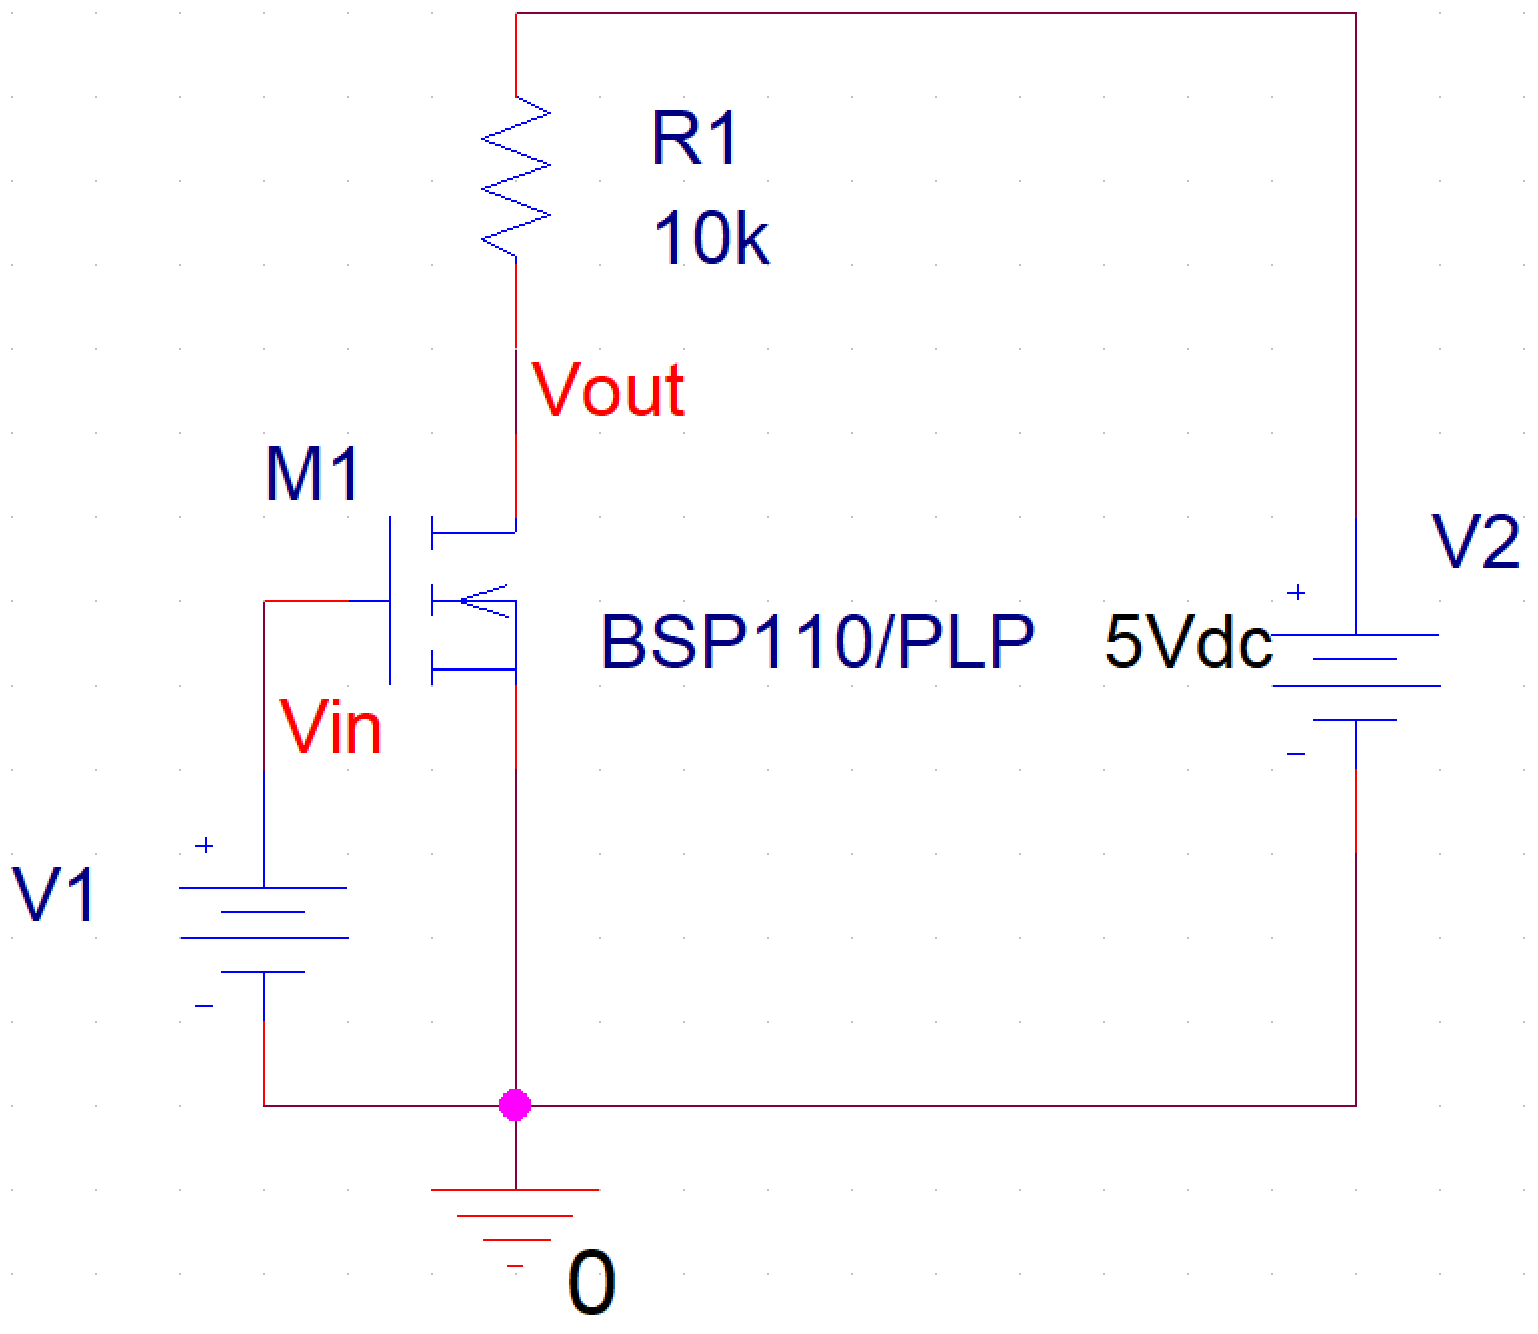
\includegraphics[width=\textwidth]{ECE2200L_Lab9_PSpice_schematic_A.png}
  \caption{PSpice simulation of MOSFET inverter circuit}
  \label{fig:ckta}
\end{figure}

\begin{figure}[H]
  \centering
  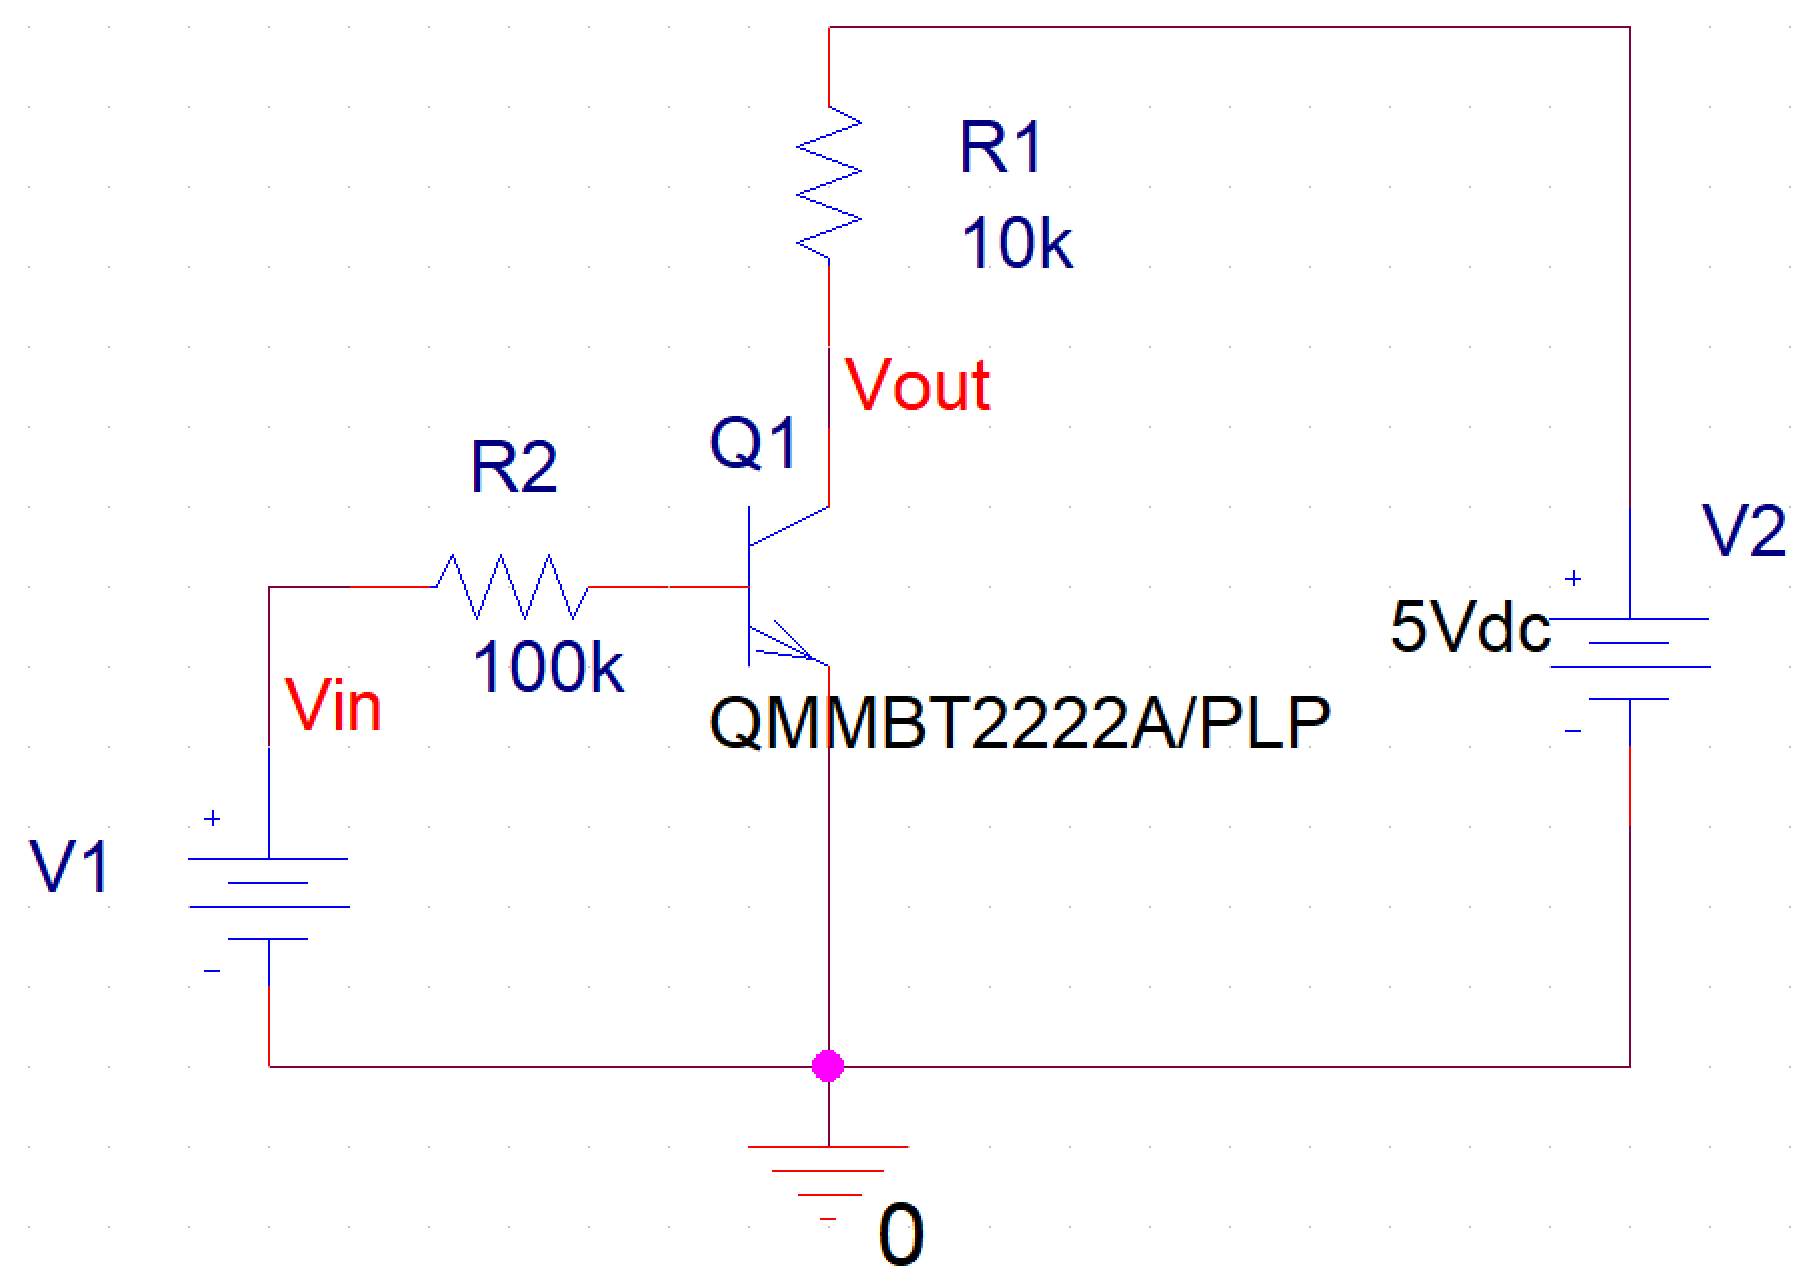
\includegraphics[width=\textwidth]{ECE2200L_Lab9_PSpice_schematic_B.png}
  \caption{PSpice simulation of BJT inverter circuit}
  \label{fig:cktb}
\end{figure}
\newpage
\begin{figure}[H]
  \centering
  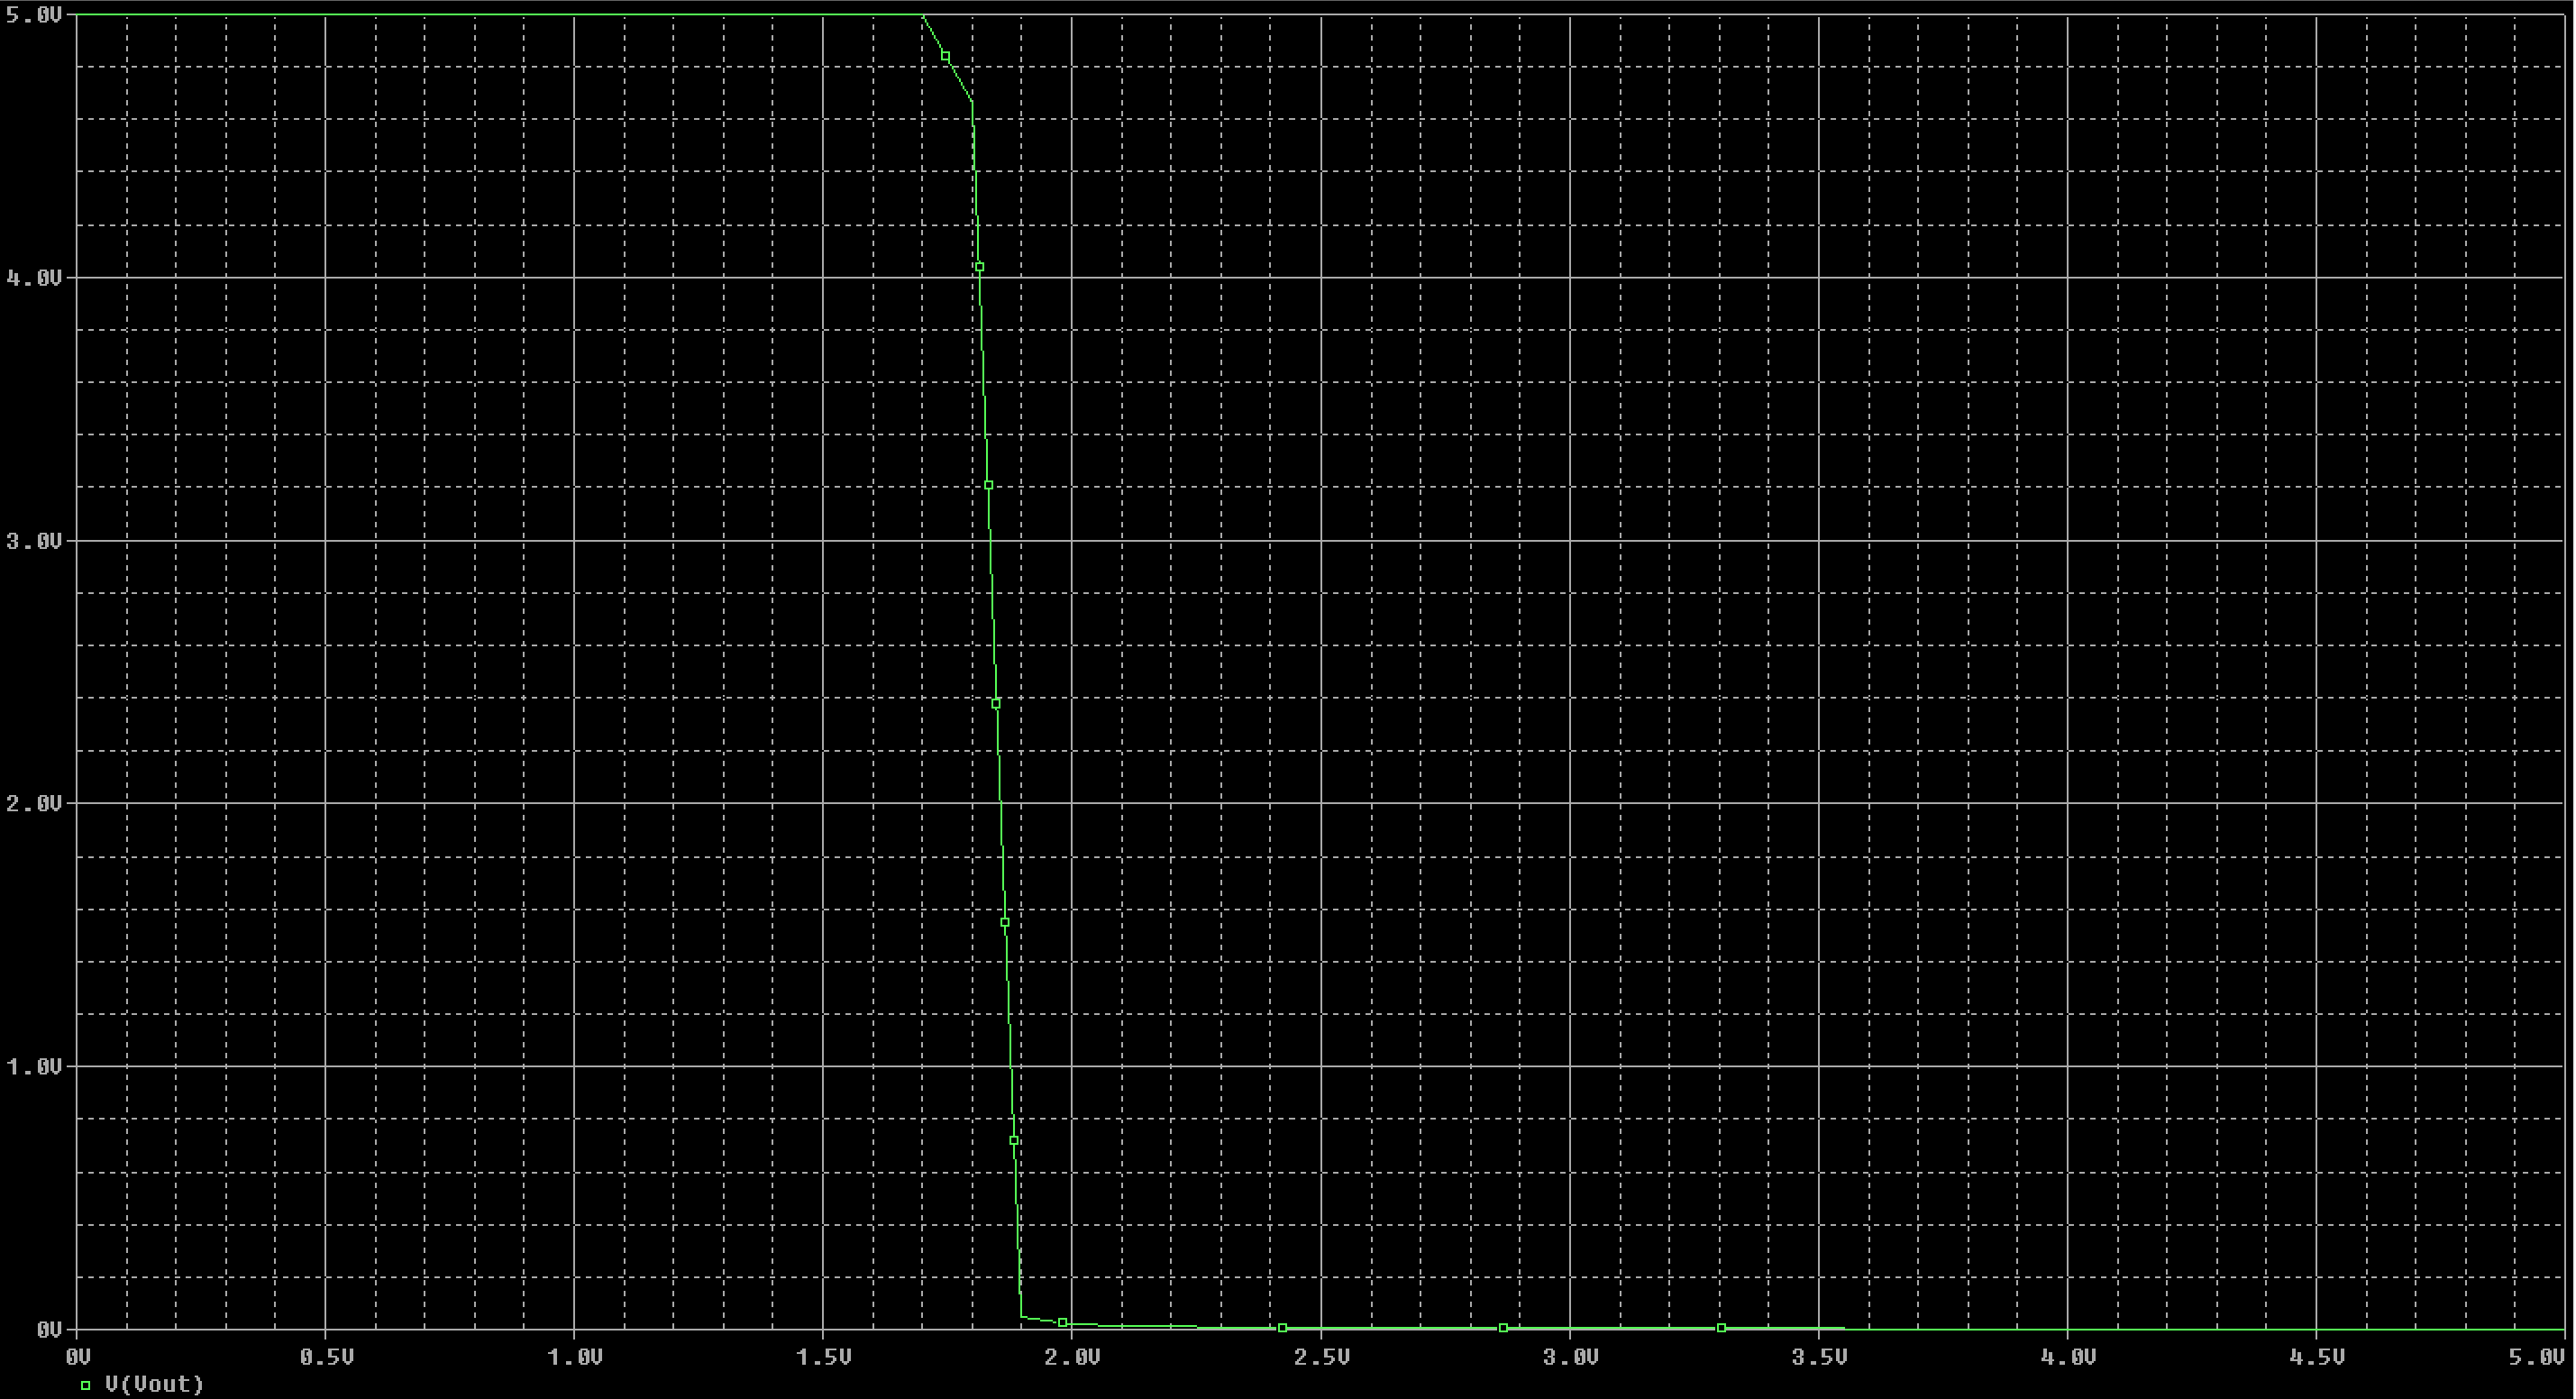
\includegraphics[width=\textwidth]{ECE2200L_Lab9_PSpice_plot_A.png}
  \caption{$V_{out}$ vs $V_{in}$ plot of MOSFET inverter circuit PSpice simulation}
  \label{fig:plota}
\end{figure}

\begin{figure}[H]
  \centering
  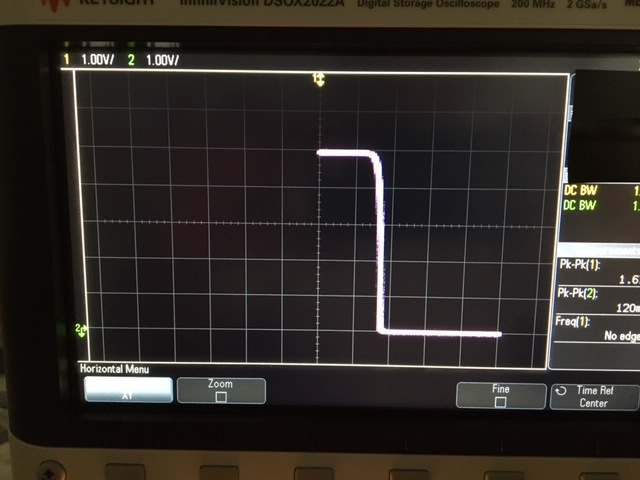
\includegraphics[width=\textwidth]{ECE2200L_Lab9_PSpice_scope_A.JPG}
  \caption{Oscilloscope $V_{out}$ vs $V_{in}$ plot of MOSFET inverter circuit}
  \label{fig:plota}
\end{figure}

\begin{figure}[H]
  \centering
  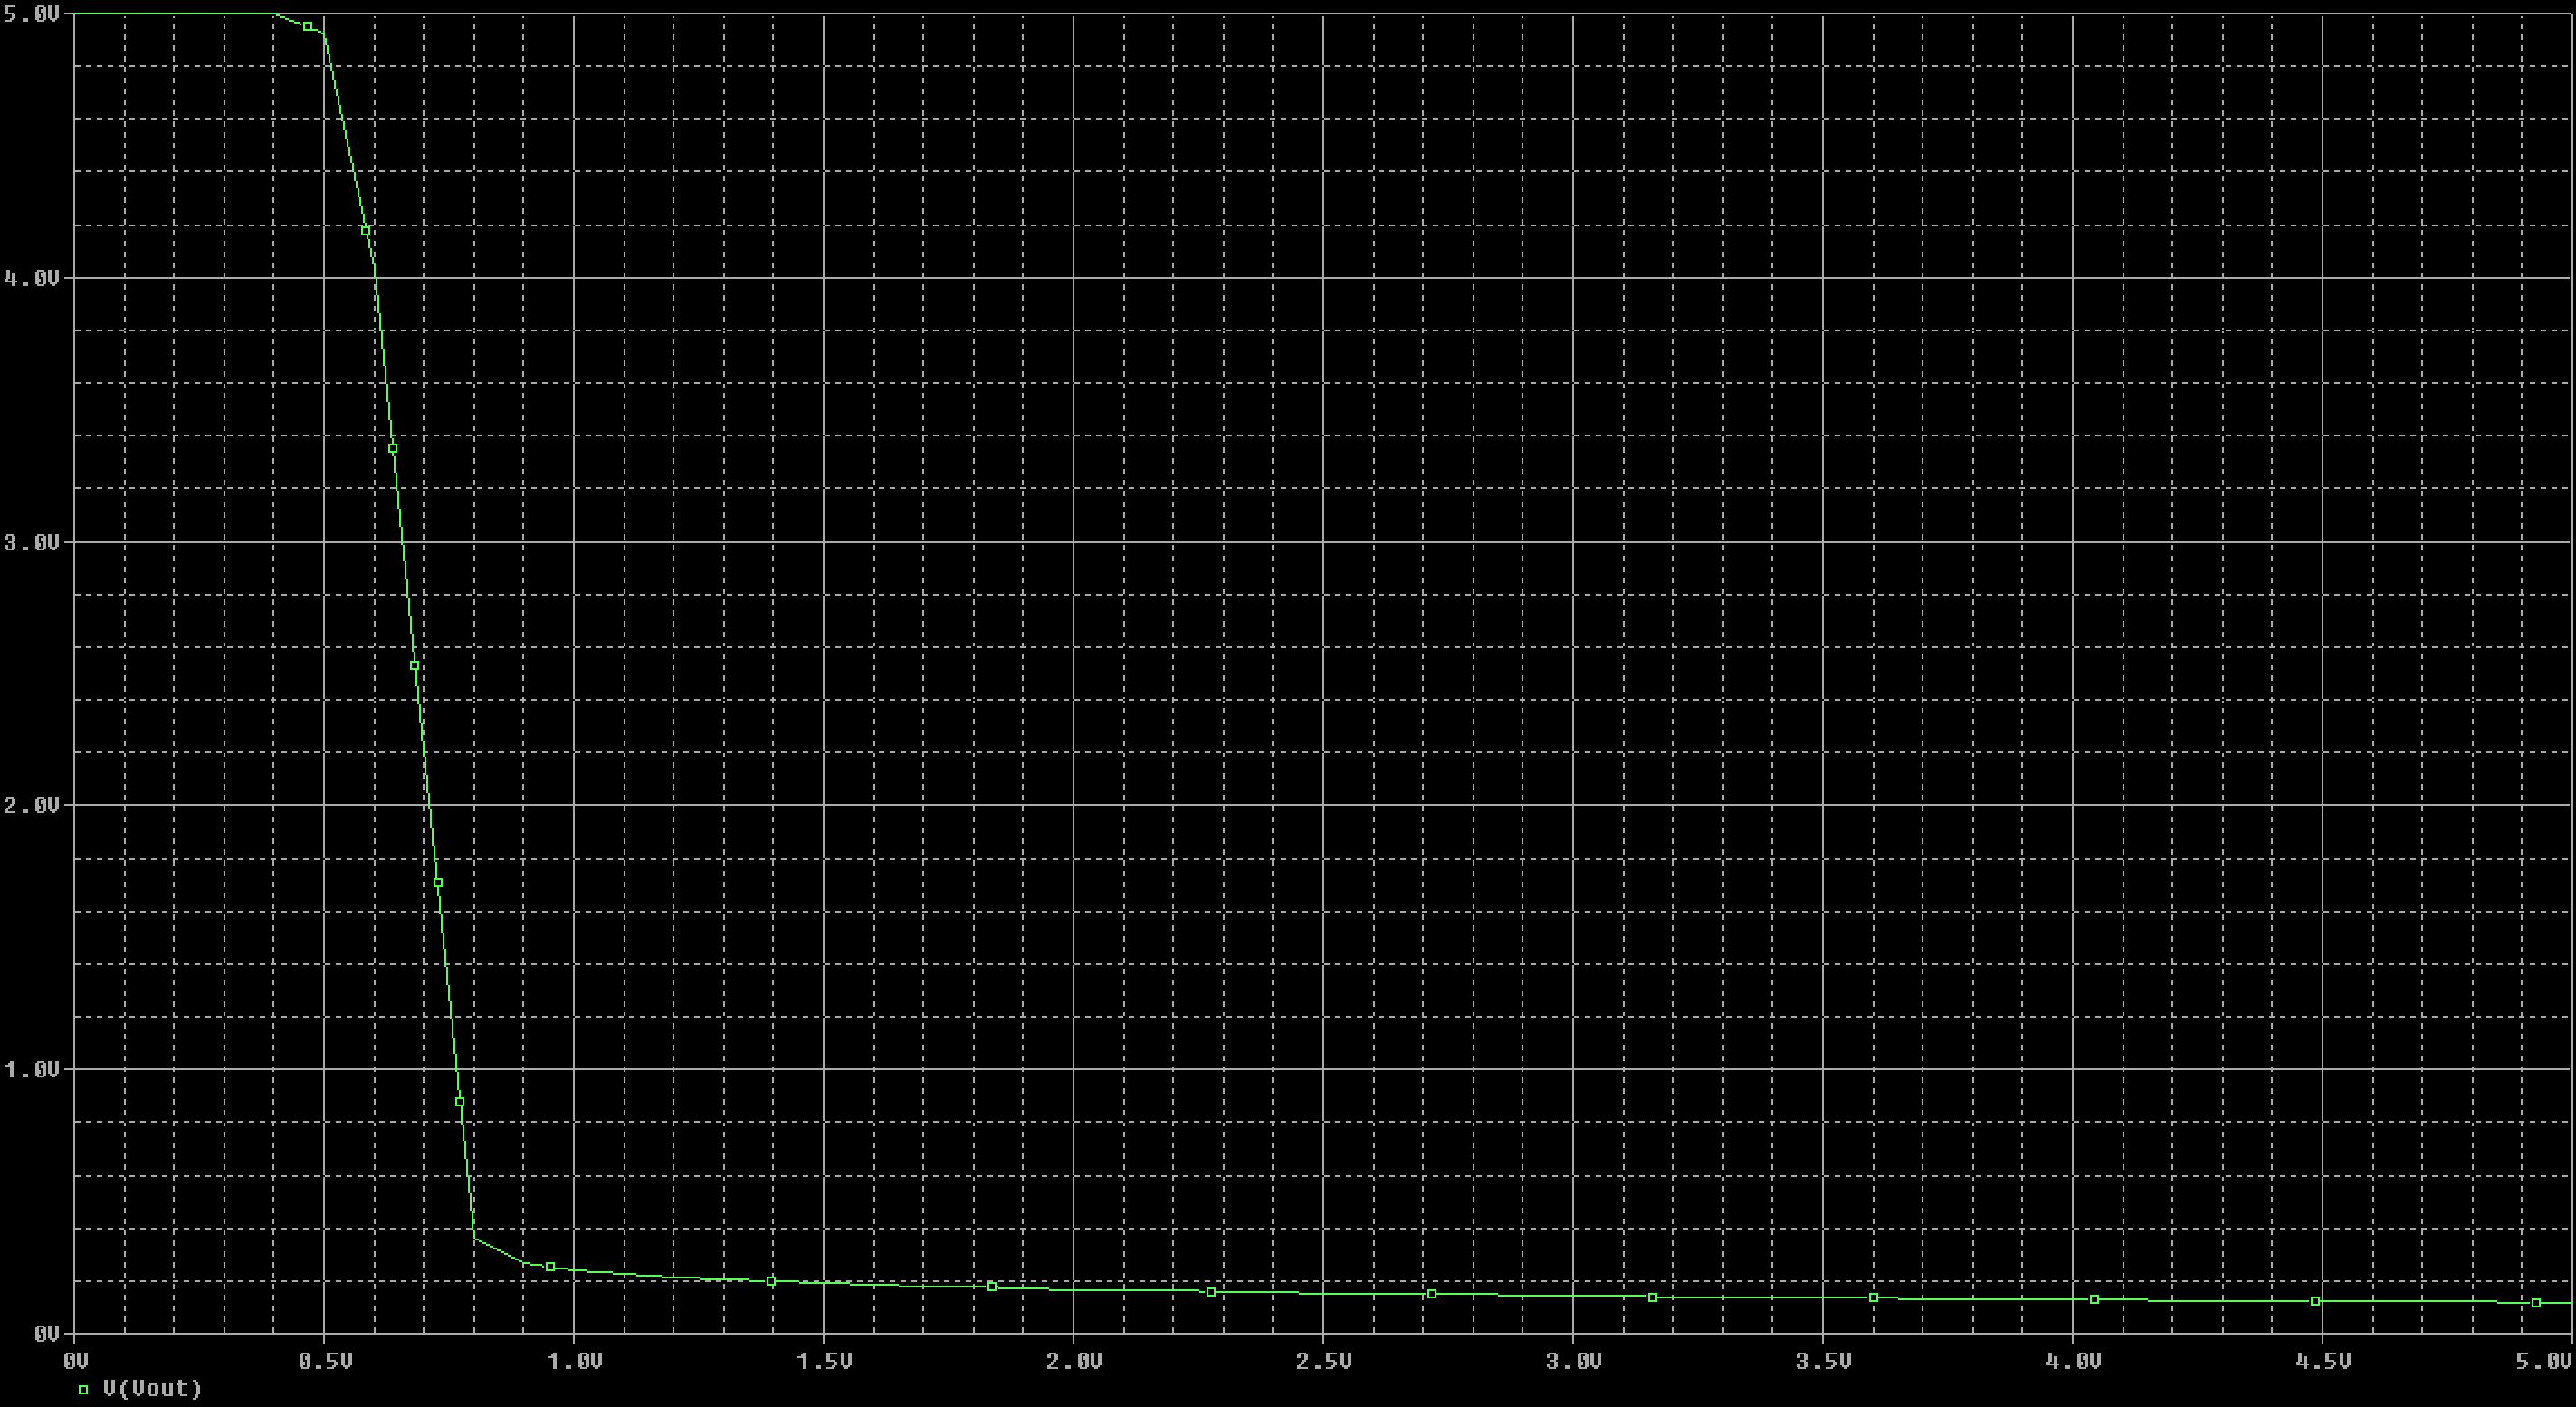
\includegraphics[width=\textwidth]{ECE2200L_Lab9_PSpice_plot_B.png}
  \caption{$V_{out}$ vs $V_{in}$ plot of BJT inverter circuit PSpice simulation}
  \label{fig:plotb}
\end{figure}

\begin{figure}[H]
  \centering
  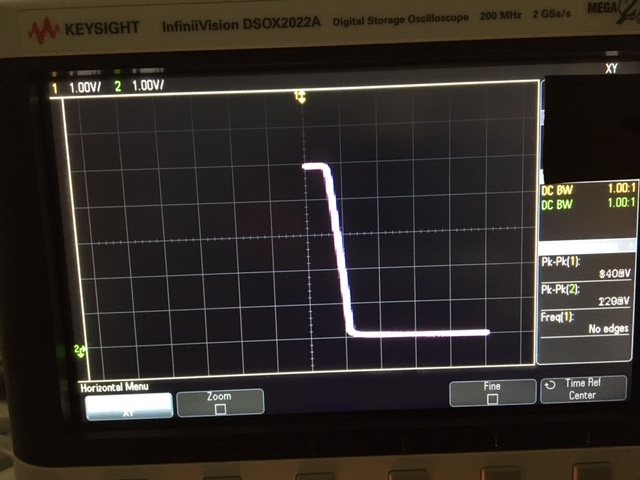
\includegraphics[width=\textwidth]{ECE2200L_Lab9_PSpice_scope_B.JPG}
  \caption{Oscilloscope $V_{out}$ vs $V_{in}$ plot of BJT inverter circuit}
  \label{fig:plotb}
\end{figure}



\section*{Conclusion}
As demonstrated above, the BJT inverter PSpice simulation $V_{out}$ vs $V_{in}$ plot shifts slightly to the left of the scope output, which could be the result of a different BJT characteristics, and the logic low voltage is higher than as shown by oscilloscope, which could be a result of low precision in oscilloscope output, but otherwise the $V_{out}$ vs $V_{in}$ plots from simulation and oscilloscope are similar for either MOSFET or BJT inverter circuit. As can be seen in the chart, the MOSFET have a larger range of $V_{in}$ values for $V_{out}$ to stigh, ay at logic hwhich is advantageous as it provide a larger tolerance to the fluctuation of input voltage levels that register as logic low from noise.
\end{document}
